\documentclass{beamer}
\usepackage{tikz,amsmath,hyperref,graphicx,stackrel}
\usetikzlibrary{positioning,shadows,arrows,shapes,calc}
\newcommand{\argmax}{\operatornamewithlimits{argmax}}
\newcommand{\argmin}{\operatornamewithlimits{argmin}}
\mode<presentation>{\usetheme{Frankfurt}}
\AtBeginSection[]
{
  \begin{frame}<beamer>
    \frametitle{Outline}
    \tableofcontents[currentsection,currentsubsection]
  \end{frame}
}
\title{Lecture 1: Review of DTFT, Gaussians, and Linear Algebra}
\author{Mark Hasegawa-Johnson}
\date{ECE 417: Multimedia Signal Processing, Fall 2020}  
\begin{document}

% Title
\begin{frame}
  \maketitle
\end{frame}

% Title
\begin{frame}
  \tableofcontents
\end{frame}

%%%%%%%%%%%%%%%%%%%%%%%%%%%%%%%%%%%%%%%%%%%%
\section[Outline]{Outline of today's lecture}
\setcounter{subsection}{1}
\begin{frame}
  \frametitle{Outline of today's lecture}
  \begin{enumerate}
  \item \href{https://courses.engr.illinois.edu/ece417/fa2020/\#syllabus}{\bf\color{blue}Syllabus}
  \item Reading: \href{http://math.mit.edu/~gs/linearalgebra/linearalgebra5_6-1.pdf}{\bf\color{blue}Strang, Section 6.1}
  \item \href{https://courses.engr.illinois.edu/ece417/fa2020/hw1.pdf}{\bf\color{blue}Homework 1}
  \item Review: DTFT, Gaussians, and Linear Algebra
  \end{enumerate}
\end{frame}

\begin{frame}
  \frametitle{What are the pre-requisites for ECE 417?}
  \begin{itemize}
  \item ECE 310 \href{https://courses.grainger.illinois.edu/ece310/fa2020/}{\bf\color{blue}Digital Signal Processing}
  \item ECE 313 \href{https://courses.grainger.illinois.edu/ece313/fa2020/}{\bf\color{blue}Probability with Engineering Applications}
  \item Math 286 \href{https://netmath.illinois.edu/college/math-286}{\bf\color{blue}Intro to Differential Eq Plus}
  \end{itemize}
\end{frame}

%%%%%%%%%%%%%%%%%%%%%%%%%%%%%%%%%%%%%%%%%%%%
\section[DTFT]{Review: DTFT}
\setcounter{subsection}{1}

\begin{frame}
  \frametitle{Discrete-Time Fourier Transform}
  The discrete-time Fourier transform of a signal $x[n]$ is
  \[
  X(\omega) = \sum_{n=-\infty}^\infty x[n]e^{-j\omega n}
  \]
  The inverse DTFT is
  \[
  x[n] = \frac{1}{2\pi}\int_{-\pi}^\pi X(\omega)e^{j\omega n}d\omega
  \]
\end{frame}

\begin{frame}
  \frametitle{DTFT of a rectangle}

  One of the most important DTFTs you should know is the DTFT of a
  length-$N$ rectangle:
  \[
  x[n] = u[n]-u[n-N]=\begin{cases}
  1 & 0\le n \le N-1\\
  0 & \mbox{otherwise}
  \end{cases}
  \]
  It is
  \[
  X(\omega)  = \sum_{n=0}^{N-1} e^{-j\omega n} =\frac{1-e^{-j\omega N}}{1-e^{-j\omega}}
  = e^{-j\omega\left(\frac{N-1}{2}\right)}\frac{\sin(\omega N/2)}{\sin(\omega/2)}
  \]
\end{frame}

\begin{frame}
  \centerline{\includegraphics[width=4.5in]{exp/img333_2x.png}}
  \centerline{\includegraphics[width=4.75in]{exp/img334_2x.png}}
  \begin{tiny}
    Smith, J.O. "The Rectangular Window", in 
    Spectral Audio Signal Processing,
    \href{http://ccrma.stanford.edu/~jos/sasp/Rectangular_Window.html}{\bf\color{blue}online book},
    2011 edition.
  \end{tiny}
\end{frame}

\begin{frame}
  \centerline{\includegraphics[width=4in]{exp/img332_2x.png}}
\end{frame}


%%%%%%%%%%%%%%%%%%%%%%%%%%%%%%%%%%%%%%%%%%%%
\section[Gaussians]{Review: Gaussians}
\setcounter{subsection}{1}

\begin{frame}
  \frametitle{Gaussian (a.k.a. normal) pdf}
  \centerline{\includegraphics[height=2in]{exp/Normal_Distribution.png}}
  \begin{tiny}
    By InductiveLoad, public domain,
    \url{https://commons.wikimedia.org/wiki/File:Normal_Distribution_PDF.svg}
  \end{tiny}
\end{frame}

\begin{frame}
  \frametitle{Normal pdf}

  A Gaussian random variable, $X$, is one whose probability density
  function is given by
  \[
  f_X(x) = \frac{1}{\sqrt{2\pi\sigma^2}}e^{-\frac{1}{2}\frac{(x-\mu)^2}{\sigma^2}}
  \]
  where $\mu$ and $\sigma^2$ are the mean and variance,
  \[
  \mu=E\left[X\right],~~~
  \sigma^2 = E\left[(X-\mu)^2\right]
  \]
\end{frame}

\begin{frame}
  \frametitle{Standard normal}

  The cumulative distribution function (CDF) of a Gaussian RV is
  \[
  F_X(x)=P\left\{X\le x\right\}
  = \int_{-\infty}^x f_X(y)dy
  = \int_{-\infty}^{(x-\mu)/\sigma} f_Z(y)dy
  = \Phi\left(\frac{x-\mu}{\sigma}\right)
  \]
  where $Z=\frac{X-\mu}{\sigma}$ is called the standard normal random
  variable.  It  is a Gaussian with zero mean, and unit variance:
  \[
  f_Z(z) = \frac{1}{\sqrt{2\pi}}e^{-\frac{1}{2}z^2}
  \]
  We define $\Phi(z)$  to be the CDF of the standard normal RV:
  \[
  \Phi(z) =  \int_{-\infty}^{z} f_Z(y)dy
  \]
\end{frame}

\begin{frame}
  \frametitle{Multivariate normal pdf}
  \centerline{\includegraphics[height=2in]{exp/MultivariateNormal.png}}
  \begin{tiny}
    By Bscan, public domain,
    \url{https://commons.wikimedia.org/wiki/File:MultivariateNormal.png}
  \end{tiny}
\end{frame}

\begin{frame}
  \frametitle{Jointly Gaussian Random Variables}

  Two random variables, $X_1$ and $X_2$, are jointly Gaussian if
  \[
  f_{X_1,X_2}(x_1,x_2) = \frac{1}{2\pi|\Sigma|^{1/2}}
  e^{-\frac{1}{2}(\vec{x}-\vec\mu)^T\Sigma^{-1}(\vec{x}-\vec\mu)}
  \]
  where $\vec{X}$ is the random vector, $\vec\mu$ is its mean, and $\Sigma$ is its
  covariance matrix,
  \[
  \vec{X}=\left[\begin{array}{c}X_1\\X_2\end{array}\right],~~~
  \vec\mu=E\left[\vec{X}\right],~~~
  \Sigma = E\left[(\vec{X}-\vec\mu)^T(\vec{X}-\vec\mu)\right]
  \]
\end{frame}

\begin{frame}
  \frametitle{Covariance}
  The covariance matrix has four elements:
  \[
  \Sigma = \left[\begin{array}{cc}\sigma_1^2 & \rho_{12} \\\rho_{21} & \sigma_2^2\end{array}\right]
  \]
  $\sigma_1^2$ and $\sigma_2^2$ are the variances of $X_1$ and $X_2$, respectively.
  $\rho_{12}=\rho_{21}$ is the covariance of $X_1$ and $X_2$:
  \begin{align*}
    \mu_1 & = E[X_1]\\
    \sigma_1^2 &= E\left[(X_1-\mu_1)^2\right]\\
    \sigma_2^2 &= E\left[(X_2-\mu_2)^2\right]\\
    \rho_{12} &= E\left[(X_1-\mu_1)(X_2-\mu_2)\right]
  \end{align*}
\end{frame}

\begin{frame}
  \frametitle{Jointly Gaussian Random Variables}
  \[
  f_{X_1,X_2}(x_1,x_2) = \frac{1}{2\pi|\Sigma|^{1/2}}
  e^{-\frac{1}{2}(\vec{x}-\vec\mu)^T\Sigma^{-1}(\vec{x}-\vec\mu)}
  \]
  The multivariate normal pdf contains the determinant and the inverse of $\Sigma$.
  For a two-dimensional vector $\vec{X}$, these are
  \begin{align*}
    \Sigma &= \left[\begin{array}{cc}\sigma_1^2 & \rho_{12} \\\rho_{21} & \sigma_2^2\end{array}\right]\\
    |\Sigma| &=\sigma_1^2\sigma_2^2 - \rho_{12}\rho_{21}\\
    \Sigma^{-1} &= \frac{1}{|\Sigma|}\left[\begin{array}{cc}
        \sigma_2^2 & -\rho_{12}\\-\rho_{21} & \sigma_1^2\end{array}\right]
  \end{align*}
\end{frame}  
  
\begin{frame}
  \frametitle{Gaussian: Uncorrelated $\Leftrightarrow$ Independent}

  Notice that if two Gaussian random variables are uncorrelated
  ($\rho_{12}=0$), then they are also independent:
  \begin{align*}
    f_{X_1,X_2}(x_1,x_2)
    &=\frac{1}{2\pi|\Sigma|^{1/2}}
    e^{-\frac{1}{2}
      \frac{\left[\begin{array}{c}x_1-\mu_1\\x_2-\mu_2\end{array}\right]^T
        \left[\begin{array}{cc}\sigma_2^2&0\\0&\sigma_1^2\end{array}\right]
        \left[\begin{array}{c}x_1-\mu_1\\x_2-\mu_2\end{array}\right]}
      {\sigma_1^2\sigma_2^2}}\\
    &=\frac{1}{2\pi\sigma_1\sigma_2}
    e^{-\frac{1}{2}\left(\frac{(x_1-\mu_1)^2}{\sigma_1^2}+\frac{(x_2-\mu_2)^2}{\sigma_2^2}\right)}\\
    &=\left(\frac{1}{\sqrt{2\pi\sigma_1^2}}e^{-\frac{1}{2}\left(\frac{x_1-\mu_2}{\sigma_1}\right)^2}\right)
    \left(\frac{1}{\sqrt{2\pi\sigma_2^2}}e^{-\frac{1}{2}\left(\frac{x_2-\mu_2}{\sigma_2}\right)^2}\right)
    \\
    &=f_{X_1}(x_1)f_{X_2}(x_2)
  \end{align*}
\end{frame}  
  
%%%%%%%%%%%%%%%%%%%%%%%%%%%%%%%%%%%%%%%%%%%%
\section[Linear Algebra]{Review: Linear Algebra}
\setcounter{subsection}{1}
\begin{frame}
  \begin{columns}[t]
    \column{2.75in}
    \begin{block}{}
      A linear transform $\vec{y}=A\vec{x}$ maps vector space $\vec{x}$
      onto vector space $\vec{y}$.  For example: the matrix
      $A=\left[\begin{array}{cc}1 & 1\\0&2\end{array}\right]$
      maps the vectors $\vec{x}_0,\vec{x}_1,\vec{x}_2,\vec{x}_3=$
      \[
      \left[\begin{array}{c}1\\0\end{array}\right],
      \left[\begin{array}{c}\frac{1}{\sqrt{2}}\\\frac{1}{\sqrt{2}}\end{array}\right],
      \left[\begin{array}{c}0\\1\end{array}\right],
      \left[\begin{array}{c}-\frac{1}{\sqrt{2}}\\\frac{1}{\sqrt{2}}\end{array}\right]
      \]
      to the vectors
      $\vec{y}_0,\vec{y}_1,\vec{y}_2,\vec{y}_3=$
      \[
      \left[\begin{array}{c}1\\0\end{array}\right],
      \left[\begin{array}{c}\sqrt{2}\\\sqrt{2}\end{array}\right],
      \left[\begin{array}{c}1\\2\end{array}\right],
      \left[\begin{array}{c}0\\\sqrt{2}\end{array}\right]
      \]
    \end{block}
    \column{1.5in}
    \begin{block}{}
      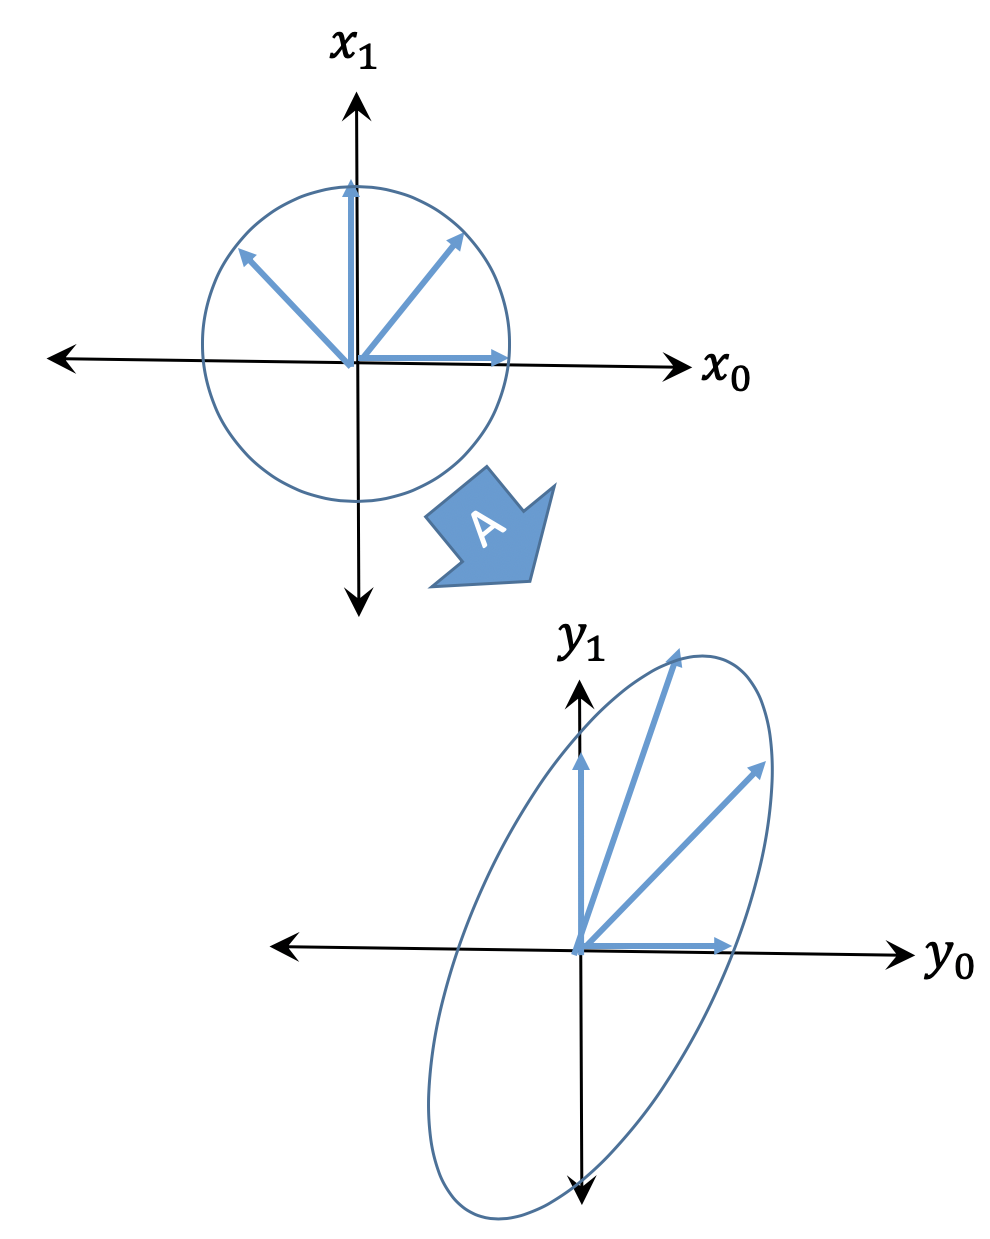
\includegraphics[width=1.45in]{linalg_review_fig1.png}
    \end{block}
  \end{columns}
\end{frame}

\begin{frame}
  \begin{columns}[t]
    \column{2.75in}
    \begin{block}{}
      A linear transform $\vec{y}=A\vec{x}$ maps vector
      space $\vec{x}$ onto vector space $\vec{y}$.  The absolute value of the
      determinant of $A$ tells you how much the area of a unit circle is
      changed under the transformation.
      
      For example, if
      $A=\left[\begin{array}{cc}1&1\\0&2\end{array}\right]$, then the
      unit circle in $\vec{x}$ (which has an area of $\pi$) is mapped to
      an ellipse with an area that is $\mbox{abs}(|A|)=2$ times larger, i.e.,
      i.e., $\pi\mbox{abs}(|A|)=2\pi$.
    \end{block}
    \column{1.5in}
    \begin{block}{}
      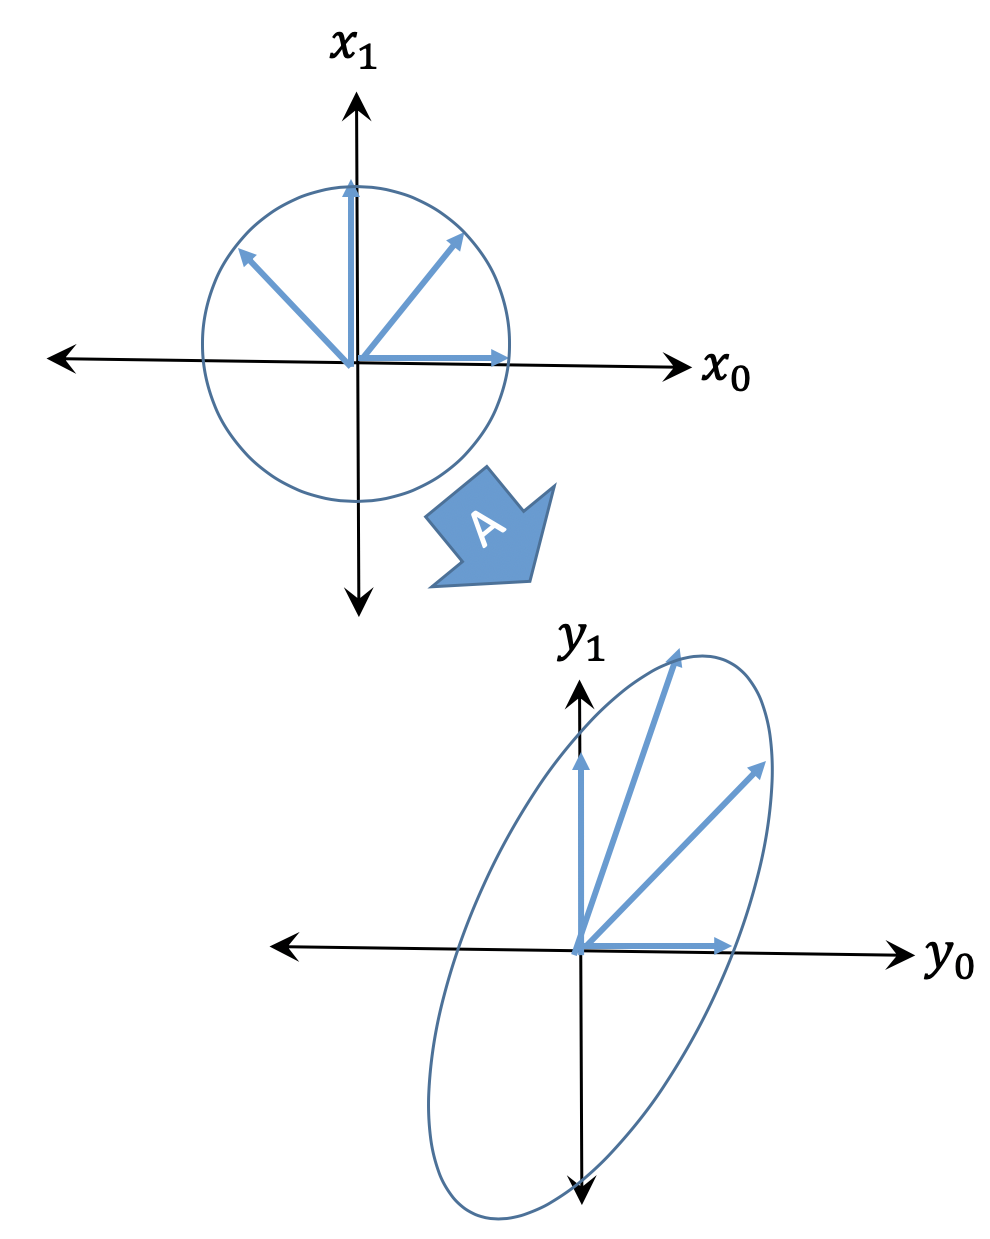
\includegraphics[width=1.45in]{linalg_review_fig1.png}
    \end{block}
  \end{columns}
\end{frame}

\begin{frame}
  \begin{columns}[t]
    \column{2.75in}
    \begin{block}{}
      For a D-dimensional square matrix, there may be up to $D$
        different directions $\vec{x}=\vec{v}_d$ such that, for some
        scalar $\lambda_d$, $A\vec{v}_d=\lambda_d\vec{v}_d$.
        For example, if
        $A=\left[\begin{array}{cc}1&1\\0&2\end{array}\right]$, then the
        eigenvectors are
        \[
        \vec{v}_0=\left[\begin{array}{c}1\\0\end{array}\right],~~
        \vec{v}_1=\left[\begin{array}{c}\frac{1}{\sqrt{2}}\\\frac{1}{\sqrt{2}}\end{array}\right],~~
        \]
        and the eigenvalues are $\lambda_0=1$, $\lambda_1=2$.
        Those vectors are red and extra-thick, in the figure to the
        left.  Notice that one of the vectors gets scaled by $\lambda_0=1$, but
        the other gets scaled by $\lambda_1=2$.
    \end{block}
    \column{1.5in}
    \begin{block}{}
      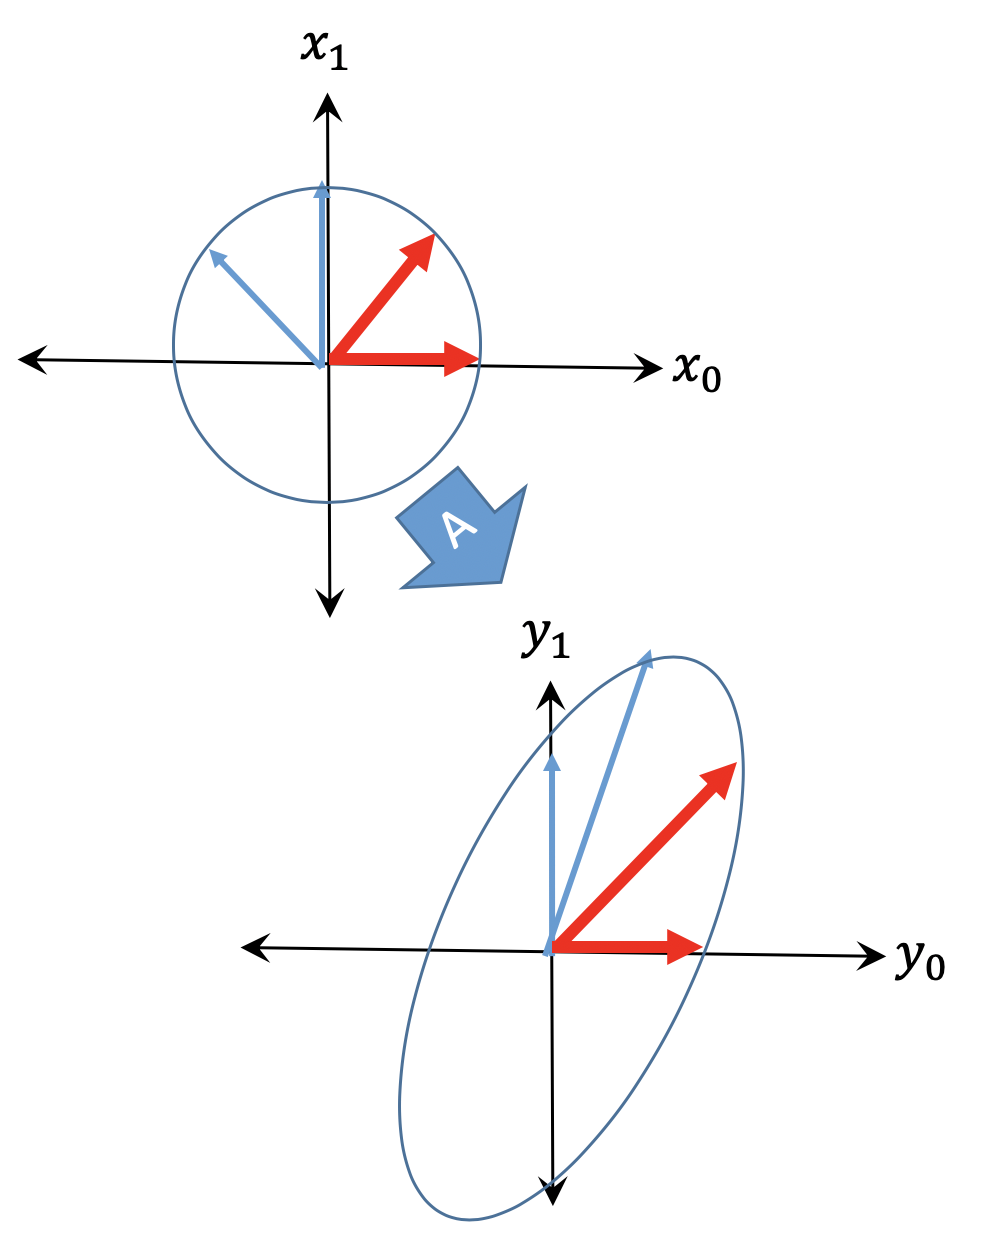
\includegraphics[width=1.45in]{linalg_review_fig2.png}
    \end{block}
  \end{columns}
\end{frame}

\begin{frame}
  \begin{columns}[t]
    \column{2.75in}
    \begin{block}{}
        An eigenvector is a direction, not just a vector.  That means
        that if you multiply an eigenvector by any scalar, you get the
        same eigenvector: if $A\vec{v}_d=\lambda_d\vec{v}_d$, then it’s
        also true that $cA\vec{v}_d=c\lambda_d\vec{v}_d$ for any scalar $c$.
        For example: the following are the same eigenvector as $\vec{v}_1$
        \[
        \sqrt{2}\vec{v}_1=\left[\begin{array}{c}1\\1\end{array}\right],~~
        -\vec{v}_1=\left[\begin{array}{c}-\frac{1}{\sqrt{2}}\\-\frac{1}{\sqrt{2}}\end{array}\right]
        \]
        Since scale and sign don't matter, by convention, we normalize so that 
        an eigenvector is always unit-length ($\Vert\vec{v}_d\Vert=1$) and
        the first nonzero element is non-negative ($v_{d0}>0$).
    \end{block}
    \column{1.5in}
    \begin{block}{}
      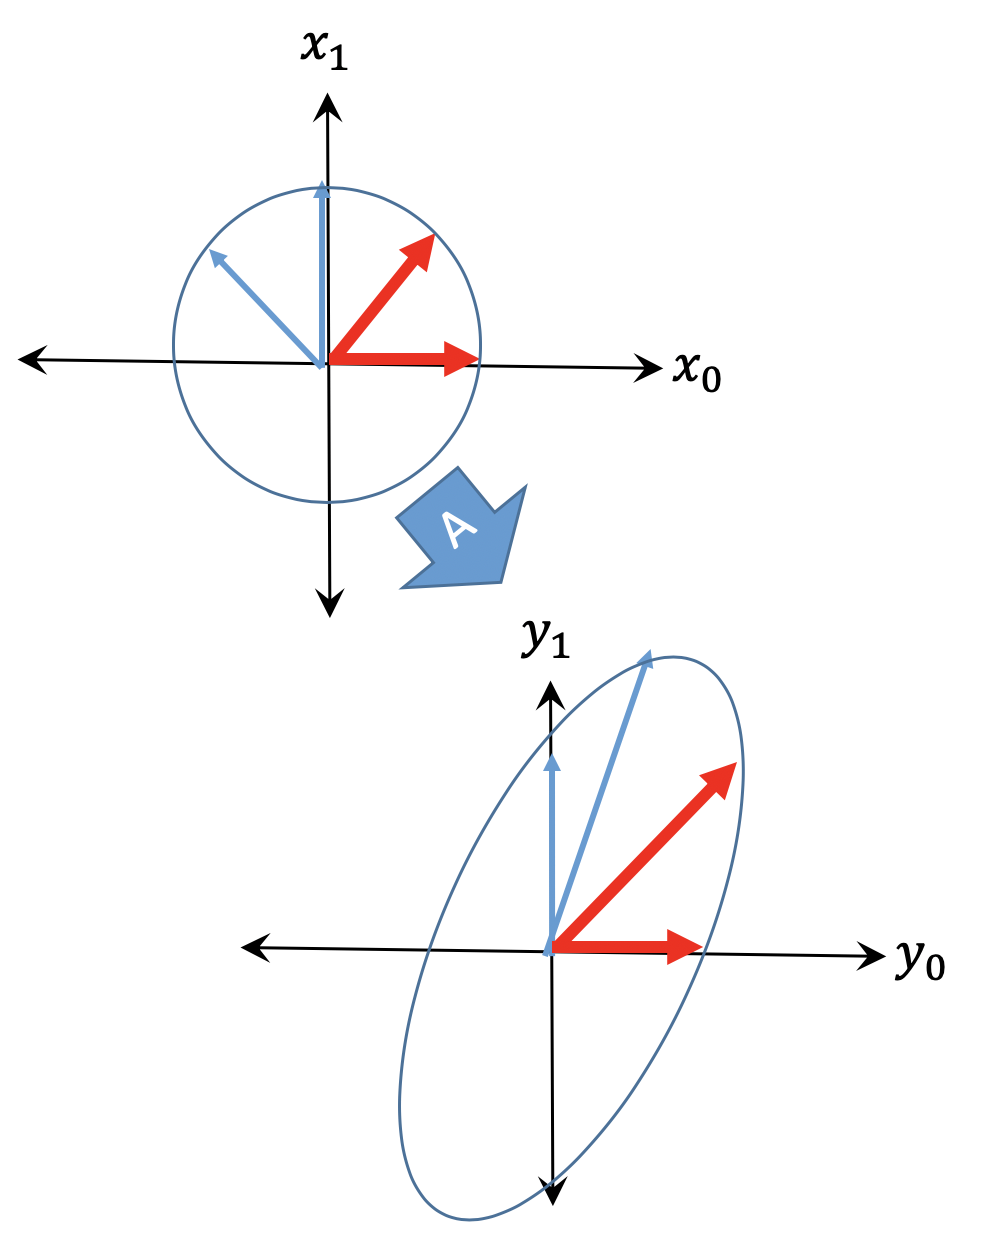
\includegraphics[width=1.45in]{linalg_review_fig2.png}
    \end{block}
  \end{columns}
\end{frame}

\begin{frame}
  \begin{columns}[t]
    \column{2.75in}
    \begin{block}{}
      \noindent{\bf Eigenvalues:}
      Before you find the eigenvectors, you should first find
      the eigenvalues.  You can do that using this fact:
      \begin{align*}
        A\vec{v}_d &= \lambda_d\vec{v}_d\\
        A\vec{v}_d &= \lambda_d I\vec{v}_d\\
        A\vec{v}_d-\lambda_d I\vec{v}_d &=\vec{0}\\
        (A-\lambda_d I)\vec{v}_d &= \vec{0}
      \end{align*}
      That means that when you use the linear transform
      $(A-\lambda_d I)$ to transform the unit circle, the result has an
      area of $|A-\lambda I|=0$.
    \end{block}
    \column{1.5in}
    \begin{block}{}
      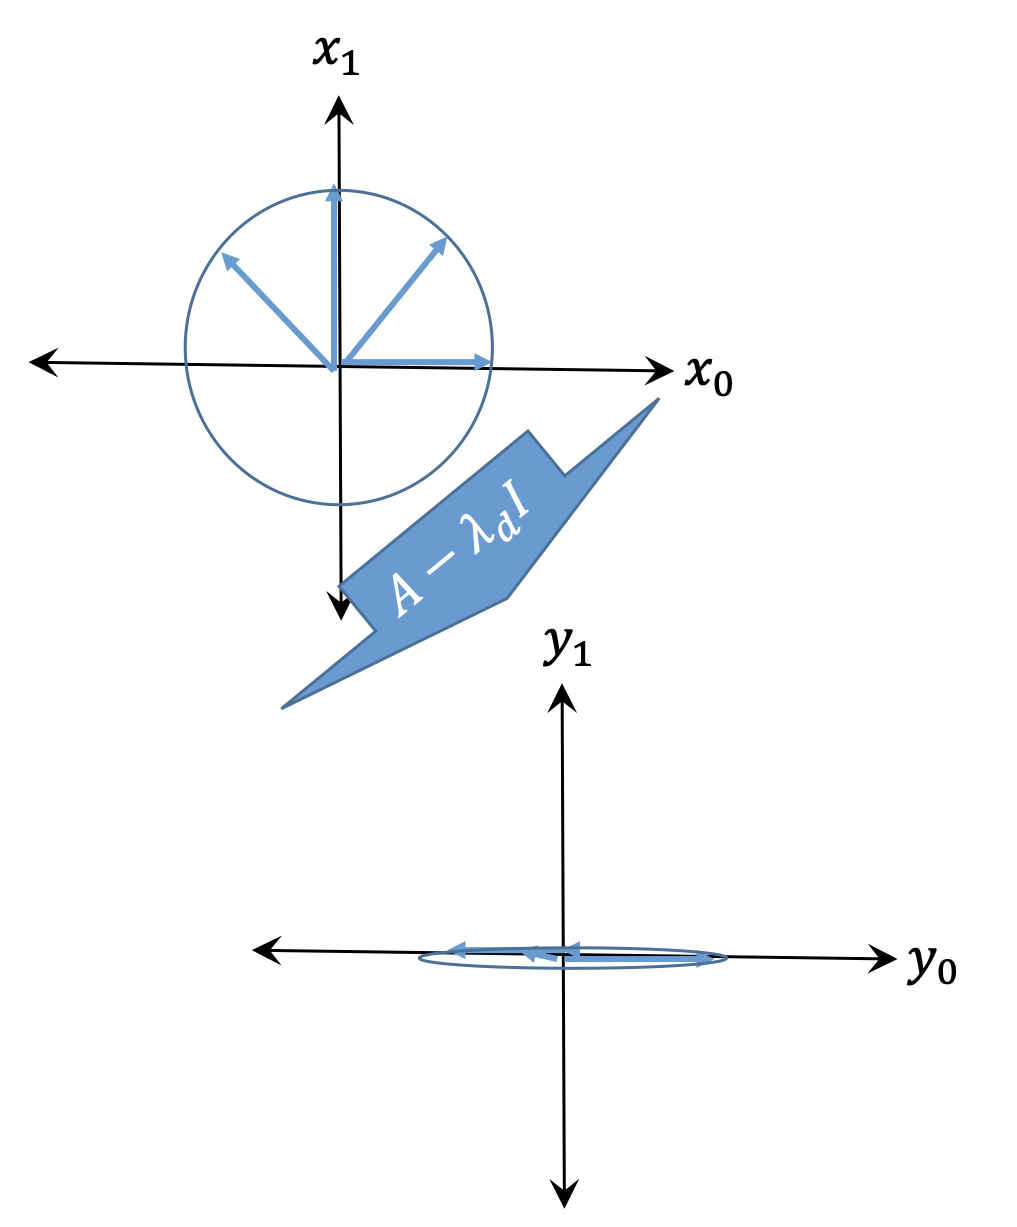
\includegraphics[width=1.45in]{linalg_review_fig3.png}
    \end{block}
  \end{columns}
\end{frame}

\begin{frame}
  \begin{columns}[t]
    \column{2.75in}
    \begin{block}{}
      \noindent{\bf Example:}
      \begin{align*}
        |A-\lambda I| &=
        \left|\begin{array}{cc}1-\lambda&1\\0&2-\lambda\end{array}\right|\\
        &=2-3\lambda+\lambda^2
      \end{align*}
      which has roots at $\lambda_0=1$, $\lambda_1=2$
    \end{block}
    \column{1.5in}
    \begin{block}{}
      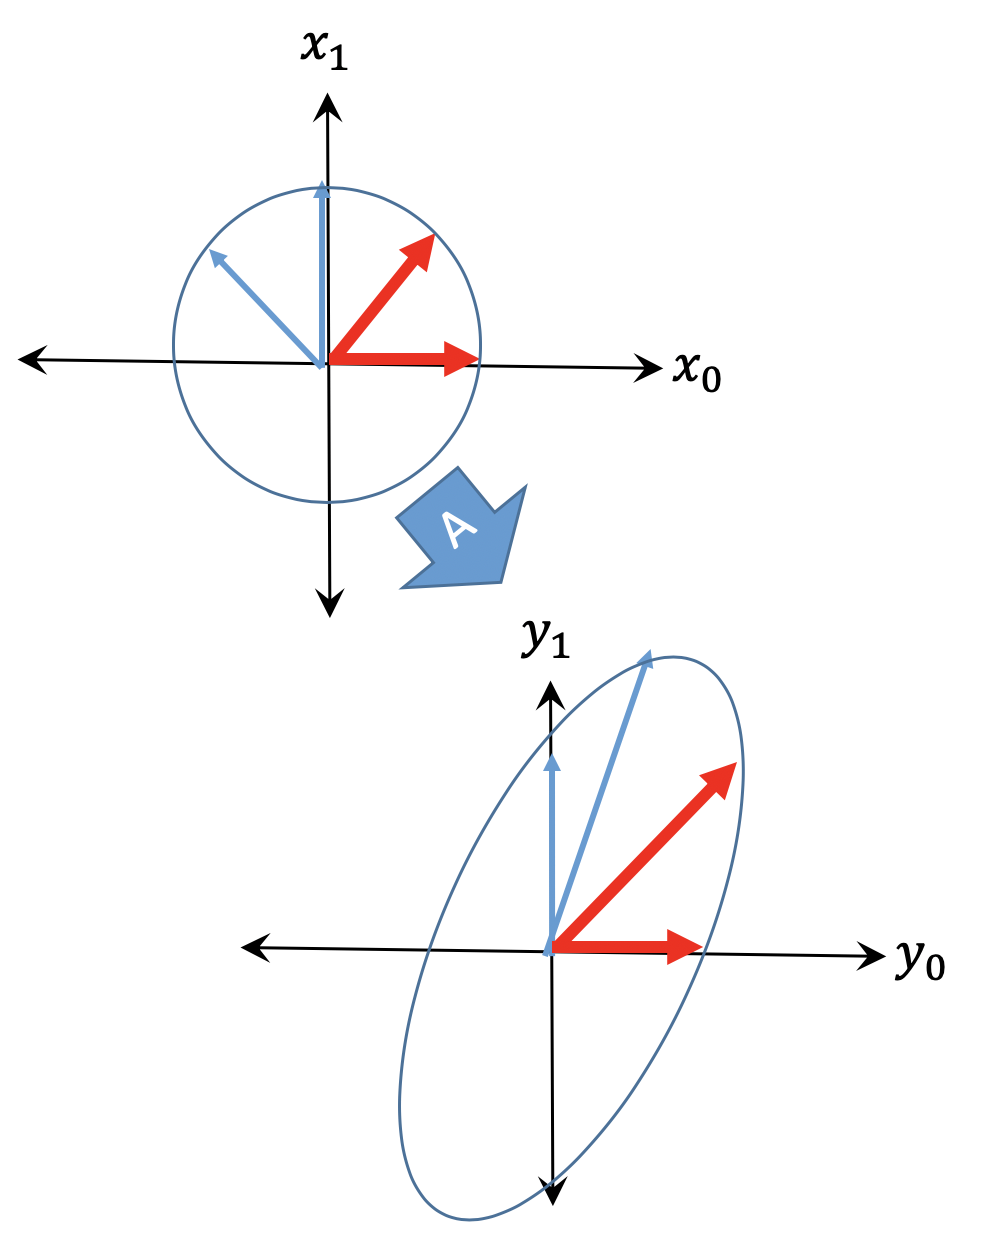
\includegraphics[width=1.45in]{linalg_review_fig2.png}
    \end{block}
  \end{columns}
\end{frame}

\begin{frame}
  \frametitle{There are always $D$ eigenvalues}
  \begin{itemize}
  \item The determinant $|A-\lambda I|$ is a $D^{\textrm{th}}$-order polynomial in $\lambda$.
  \item By the fundamental theorem of algebra, the equation
    \[
    |A-\lambda I|=0
    \]
    has exactly $D$ roots (counting repeated roots and complex roots).
  \item Therefore, {\bf any square matrix has exactly $D$ eigenvalues}
    (counting repeated eigenvalues, and complex eigenvalues.
  \item The same is not true of eigenvalues.  {\bf Not every square
    matrix has eigenvectors}.  Complex and repeated eigenvalues
    usually correspond to eigensubspaces, not eigenvectors.
  \end{itemize}
\end{frame}

\section{Summary}
\begin{frame}
  \frametitle{Summary}
  \begin{itemize}
    \item DTFT of a rectangle: 
      \[
      x[n]=u[n]-u[n-N] \leftrightarrow
      X(\omega)=e^{-j\omega\left(\frac{N-1}{2}\right)}\frac{\sin(\omega N/2)}{\sin(\omega/2)}
      \]
    \item Jointly Gaussian RVs:
      \[
      f_{\vec{X}}(\vec{x}) = \frac{1}{2\pi|\Sigma|^{1/2}}
      e^{-\frac{1}{2}(\vec{x}-\vec\mu)^T\Sigma^{-1}(\vec{x}-\vec\mu)}
      \]
    \item Linear algebra:
      \[
      |A-\lambda I|=0,~~~A\vec{v}=\lambda\vec{v}
      \]
  \end{itemize}
\end{frame}

\end{document}

